% !TEX encoding = UTF-8
% !TEX program = pdflatex
% !TEX root = MEMOC.tex
% !TEX spellcheck = it-IT

% 6 Ottobre 2016

\chapter{Introduzione}

Il corso è in inglese, ma il contenuto non cambia rispetto l'anno scorso. Anche il materiale fornito sarà in inglese. La mail del docente è \url{luigi@math.unipd.it}. C'è anche il professore Di Summa che farà il laboratorio.

La pagina del corso è \url{http://www.math.unipd.it/~luigi/courses/metmodoc/metmodoc.html}.

\section{Obiettivo del corso}

L'obiettivo del corso è quello di introdurre delle tecniche avanzate per la modellazione e risoluzione di problemi di ottimizzazione combinatoria.
Si tratta di problemi in cui si vuole ottimizzare un certo criterio trovando una combinazione ottima di risorse da utilizzare.

Il corso vuole fornire gli strumenti matematici e algoritmici per risolvere questo tipo di problemi, concentrandosi per lo più su problemi pratici, che verranno risolti utilizzando vari software.

Un esempio di problemi è dato da quello del telefono, ci sono delle risorse limitate per creare due possibili modelli di telefoni che vengono commercializzati a prezzi diversi. Si vuole trovare il numero di telefoni di ciascun modello da produrre per ottenere il maggior guadagno possibile in funzione delle risorse a disposizione.

\begin{figure}[htbp]
\centering
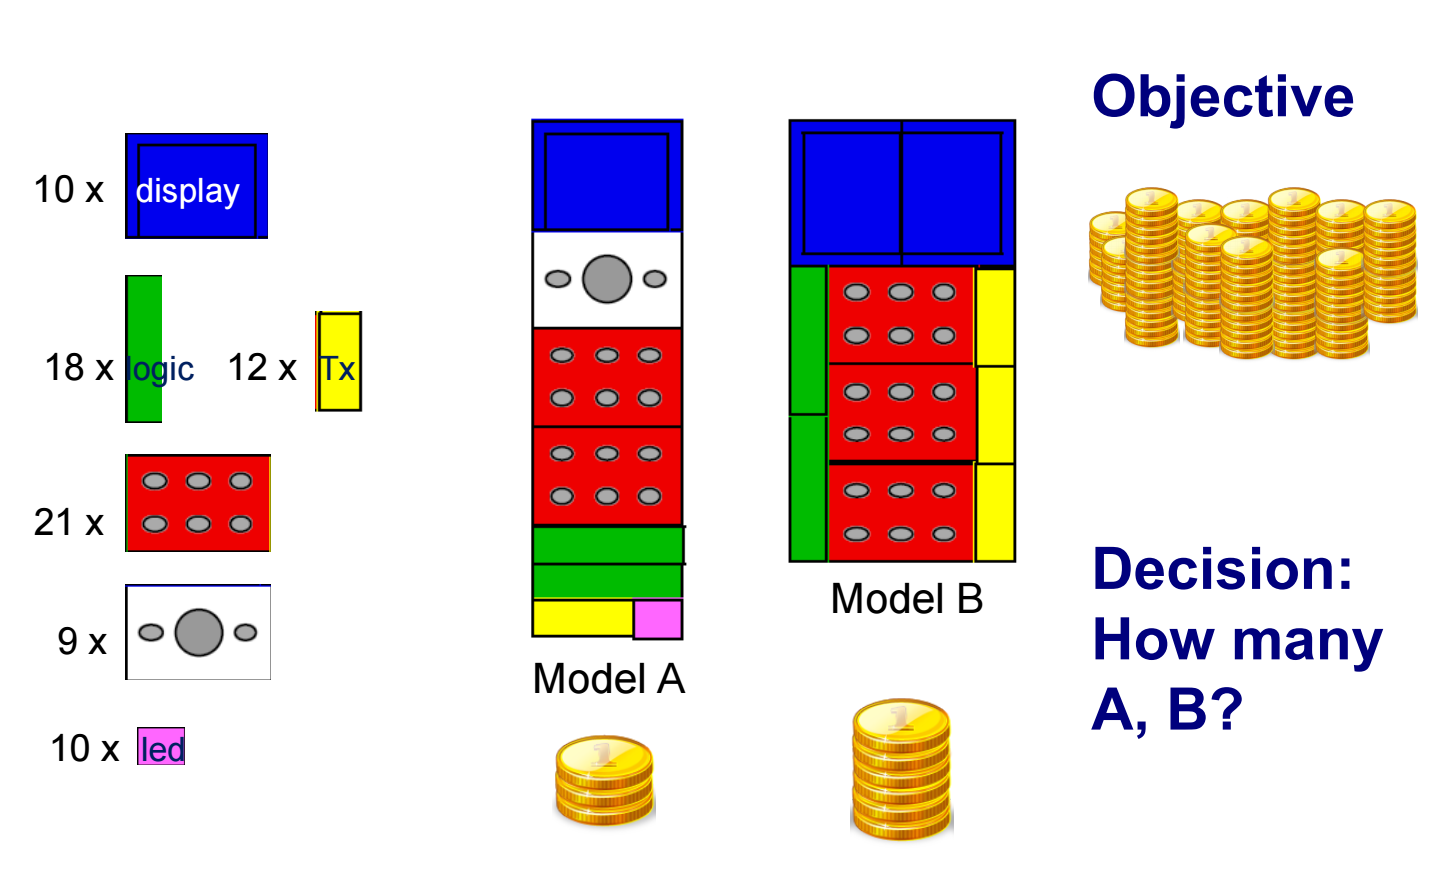
\includegraphics[width=0.7\textwidth]{images/l1-telefono.png}
\end{figure}

Per risolvere questo problema si possono usare varie strategie:

\begin{itemize}
	\item \textbf{Greedy}: scelgo di costruire il massimo numero di telefoni del modello con il prezzo più alto. Però non ho la garanzia che la soluzione trovata sia ottima.
	\item \textbf{Local search}: determino un certo numero di telefoni da produrre in modo da trovare una possibile soluzione sub-ottima per poi andare a modificare il numero di telefoni prodotti, cercando di migliorare il guadagno. Anche in questo caso non ho la garanzia che la soluzione trovata sia ottima.
	\item \textbf{Global search}: provo tutte le possibili combinazioni di telefoni che posso produrre, così facendo sono sicuro di trovare una soluzione ottima.
\end{itemize}


Un altro possibile problema è quello del contadino che possiede 12 ettari di terra dove può coltivare patate o pomodori, avendo a disposizione 70kg di semi di pomodoro, 18 tonnellate di tuberi di patate e 160 tonnellate di fertilizzante. Il contadino sa che un ettaro di campo coltivato a pomodori produce un guadagno di 3000 euro mentre uno di patate 5000. Per coltivare un ettaro a pomodori servono 7kg di semi e 10 tonnellate di fertilizzante, mentre un ettaro di patate richiede 3 tonnellate di tuberi e 20 di fertilizzante.

Questo problema è simile a quello del telefono, con la differenza che in questo caso gli ettari possono essere frazionati e quindi l'approccio combinatorio non può essere utilizzato.

L'idea è quindi quella di formulare un modello che descrive la soluzione ottima, anziché formulare un algoritmo che lo risolve.

Come prima cosa è necessario identificare le \textbf{variabili decisionali}, in questo caso $x_T$ e $x_P$ che rappresentano gli ettari coltivati. 
Poi si deve definire la \textbf{funzione obiettivo} che si vuole ottimizzare, in questo caso $\max 3000 x_T + 5000 x_P$.
Infine è necessario definire i \textbf{vincoli del problema} per modellare il consumo di risorse. In questo caso:

\begin{align*}
	x_T + x_P &\leq 12 \text{ vincolo sulla terra} \\
	7 x_T &\leq 70   \text{ vincolo sui semi di pomodoro} \\
	3 x_P &\leq 18 \text{ vincolo sui tuberi} \\
	10 x_T + 20 x_P &\leq 160 \text{ vincolo sul fertilizzante} 
\end{align*}

Con questa formulazione del problema non dico niente riguardo la soluzione del problema, ma posso utilizzare il modello creato per trovarla utilizzando dei metodi matematici dato che l'insieme di vincoli può essere visto come un sistema di disequazioni.

Un primo approccio è quello di partire da un valore di partenza della funzione obiettivo, ad esempio 27000 e provare a migliorarlo utilizzando la discesa di gradiente, fino a trovare un punto del piano che corrisponde ad un valore ottimo.
Con questo approccio posso anche dire che la soluzione trovata è ottima, perché tutte le altre soluzioni migliori richiedono un maggior numero di risorse.

\begin{figure}[htbp]
	\centering
	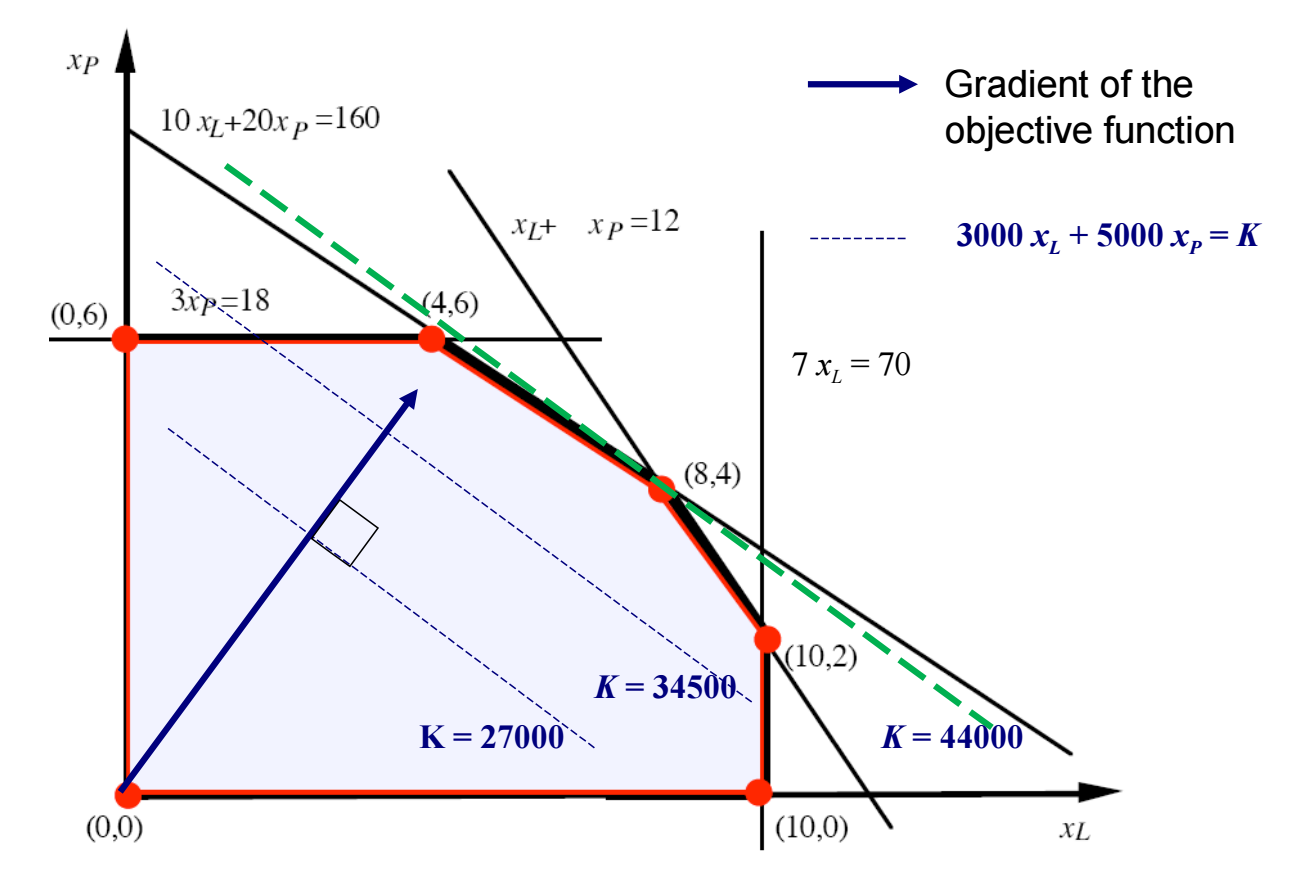
\includegraphics[width=0.5\textwidth]{images/l1-poligono.png}
\end{figure}


Tutto questo funziona perché sia i vincoli che la funzione obiettivo sono \textbf{lineari} e le variabili sono numeri reali. Questo tipo di modelli prende quindi il nome di \textbf{Linear Programming}.

Da notare che in questo caso la soluzione ottima è su un vertice intero, ma è un caso. Se le variabili utilizzate possono essere solo intere la situazione diventa più complessa perché è necessario effettuare delle approssimazioni.

\section{Approccio della ricerca operativa}

\begin{figure}[htbp]
	\centering
	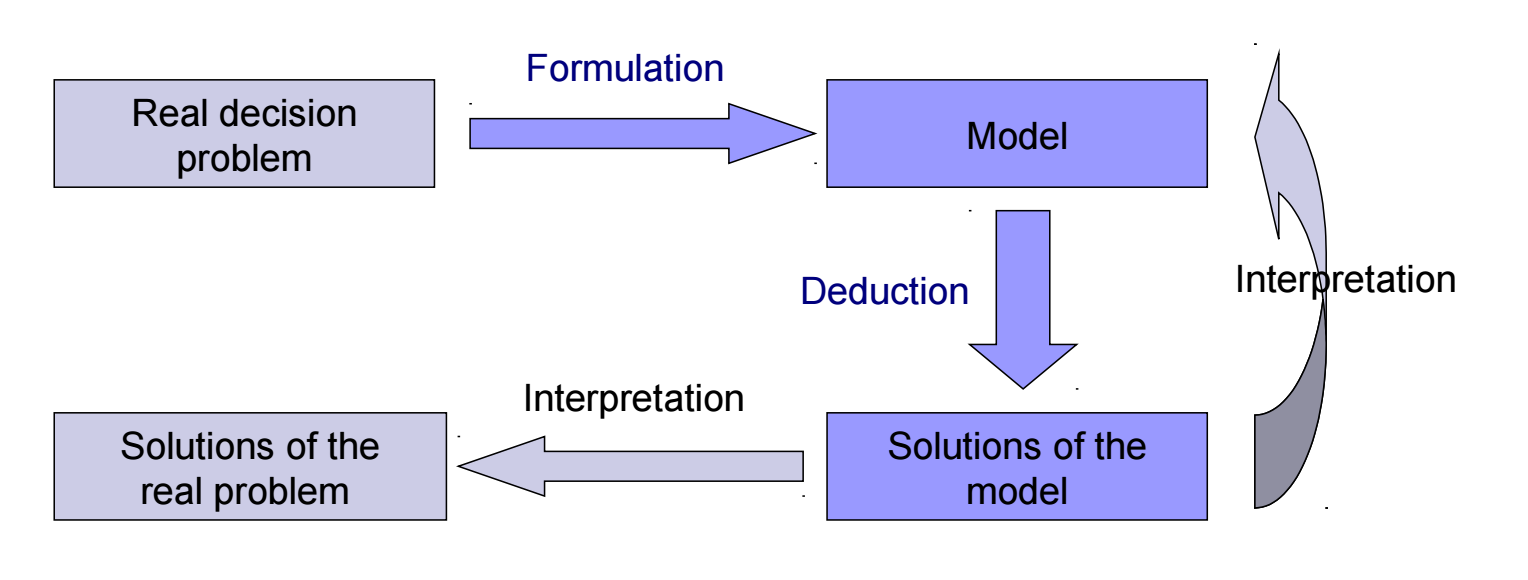
\includegraphics[width=0.7\textwidth]{images/l1-approccio.png}
\end{figure}

L'approccio precedentemente descritto è quello della ricerca operativa: si parte da un problema reale che viene formalizzato utilizzando un modello. Dal modello viene trovata una soluzione ottima per esso, la quale deve poi essere trasformata nella soluzione del problema reale.
Questo secondo passo può essere necessario perché nel modellare il problema può essere che sia stato necessario modificare alcuni vincoli, oppure utilizzare delle variabili reali anziché intere.

Si possono quindi definire due fasi: una di \textbf{formulazione} del modello e una di \textbf{deduzione} della soluzione, utilizzando alcuni algoritmi già definiti o personalizzati.

\section{Programma del corso}

\begin{enumerate}
	\item Ripasso e approfondimento delle tecniche di programmazione lineare e della dualità.
		\begin{itemize}
			\item Modelli LP, metodo del simplesso, teorema della dualità.
			\item Column generation technique per modelli LP grandi. Ovvero la creazione di modelli dinamici per evitare le limitazioni della memoria.
			\item Applicazioni: pianificazione della produzione, gestione del flusso di rete.
		\end{itemize}
	\item Metodi avanzati per la programmazione lineare intera mista (\textbf{MILP}).
		\begin{itemize}
			\item Formulazioni alternative, Branch \& Bound, Branch \& Cut.
			\item Applicazioni: Traveling Salesman Problem, localizzazione dei magazzini, set cover.
		\end{itemize}
	\item Meta euristiche per l'ottimizzazione combinatoria.
		\begin{itemize}
			\item Neighbourhood search e varianti.
			\item Algoritmi genetici.
		\end{itemize}
	\item Network optimization: modellazione dei problemi di ottimizzazione con i grafi. \textit{Potrebbe non essere affrontato.}
	\item \textbf{Laboratorio}:
		\begin{itemize}
			\item Online optimization server
			\item Optimization software and Algebraic modelling languages
			\item Optimization libraries (Cplex, Coin-OR, Scip)
		\end{itemize}
\end{enumerate}


\section{Informazioni pratiche}

Ci saranno dei laboratori nell'orario delle lezioni, verrà specificato nel sito quando ci saranno.

Non ci sono libri, vengono fornite le dispense dal professore e saranno in inglese.

Per ottenere il software che verrà utilizzato il laboratori è necessario registrarsi sul sito \url{http://www.math.unipd.it/userlist/subscribe/?idlist=277}, utilizzando la chiave \texttt{MeMoCO.16}. Per scaricare gratuitamente CPlex Optiumization Suite è necessario registrarsi alla IBM Academic Initiative.

L'esame è composto da:

\begin{itemize}
	\item Due esercitazioni di laboratorio, una sulla modellazione MILP e una sulle meta-euristiche, da consegnare qualche giorno prima dell'orale. Da fino a 10 punti.
	\item Esame orale che consiste nella discussione delle esercitazioni di laboratorio e delle domande teoriche sui contenuti del corso. Da fino a 20 punti. Forse si può fare in italiano.
	\item Progettino opzionale per ottenere un bonus da 2 a 6 punti. Il progetto riguarda la modellazione di un problema accordato con il docente e risolto utilizzando delle meta-euristiche o in modo esatto. Può essere fatto anche dopo lo scritto.
\end{itemize}


